\title{Project 2: Continuous Control}
\author{
	Rory McGrath \\
}
\date{\today}

\documentclass[12pt]{article}
\usepackage[margin=1in]{geometry}
\usepackage{graphicx}
\usepackage[backend=bibtex,style=numeric]{biblatex}
\bibliography{References}
\usepackage[table]{xcolor}

\begin{document}
\maketitle


\section{Overview}
In this environment, a double-jointed arm acts as the agent and can move to target locations.
A reward of +0.1 is provided for each step that the agent's hand is in the goal location. 
The objective of the agent is to maintain its position at the target location for as many time steps as possible.

The observation space consists of 33 variables corresponding to position, rotation, velocity, and angular velocities of the arm. 
Each action is a vector with four numbers, corresponding to torque applicable to two joints. 
Every entry in the action vector should be a number between -1 and 1.
This task is episodic,  in order to solve the environment the agent must achieve an average score of +30 over 100 consecutive episodes.

\section{Methods}
\label{methods}
An Actor-Critic approach was used to solve this problem.
A value based method such as Deep Q Networks (DQN) \cite{dqn_paper} could have been adapted but it would require discretising the action space. 
Depending on the required granuality of the descretisation and the degrees of freedom in the arm this would lead to a rapidly growing action space \cite{curse_of_dimensionality}.
With this limitation in mind an Actor-Critic algorithm Deep Deterministic Policy Gradients (DDPG)\cite{ddpg_paper} was implemented.

Similar to DQN, DDPG uses deep artifical neural networks as large non-linear function approximators for the value function.
In order to train these function approximators in a stabe and robust way DDPG also uses a Replay Buffer\cite{experience_replay} and updates the target networks with "soft target updates" \cite{ddpg_paper}.
The DDPG maintains four seperate ANNs.
Two are the local and target actor functions and two are the local and target critic functions.
The actor function $\mu(s|\theta^{\mu})$ specifies the current policy by deterministically mapping states to a specific action.
The critic function $Q(s,a)$ is learned using the Bellman equation.

One issue with learning in continuous space is exploration.
How does the agent explore the environment?
Given that this is an off-policy algorithm we can construct an exploration policy $\mu'$ by adding noise sampled from a noise process $N$.
Adding this noise to the actor policy yields an exploration policy:
$$\mu'(s_t) = \mu(s_t|\theta_t^\mu) + N$$

When observing the behaviour of the trained agent this exploration can be turned off.

\section{Results}
Using the methodology described above [\ref{methods}] an agent was trained to solve the environment.
The agent was written in pyTorch and was run using the openai gym toolkit.

The ANN used for the actor consisted of an input layer of 33 nodes, one dense hidden layer of 33 nodes and an output layer of 4 nodes.
The activation functions for the input and hidden layer was the rectified linear units (ReLUs). 
The output layers activation function was the hyperbolic tangent function (tanh). 
This maps the output to a range between -1 and 1 which is the required input for the motors

The ANN used for the critic has a similar arthecture and consisted of an input layer of 33 nodes, one dense hidden layer of 33 nodes and an output layer of 1 node.

The following hyper-parameters were used to train the agent:


\begin{table}[h!t]
\begin{minipage}{.5\linewidth}
\begin{tabular}{|c|l|}
	\hline
	\multicolumn{2}{|c|}{\textbf{Learning Updates}}\\
	\hline
	\hline
	\textbf{Parameter} & \textbf{Value}\\
	\hline
	$\gamma$ & $0.99$\\
	$\alpha$ & $5e^{-4}$\\
	\hline
\end{tabular}
\end{minipage}
\begin{minipage}{.5\linewidth}
\begin{tabular}{|c|l|}
	\hline
	\multicolumn{2}{|c|}{\textbf{Experience Replay}}\\
	\hline
	\hline
	\textbf{Parameter} & \textbf{Value}\\
	\hline
	Buffer Size & $1e^{5}$\\
	Batch Size & $64$\\
	\hline
\end{tabular}
\end{minipage}
\end{table}
\begin{table}
\begin{minipage}{.5\linewidth}
\begin{tabular}{|c|l|}
	\hline
	\multicolumn{2}{|c|}{\textbf{Actor Network}}\\
	\hline
	\hline
	\textbf{Parameter} & \textbf{Value}\\
	\hline
		$\tau$ & $1e^{-3}$\\
		Update Rate & every 4 time-steps \\
	\hline
\end{tabular}
\end{minipage}
\begin{minipage}{.5\linewidth}
\begin{tabular}{|c|l|}
	\hline
	\multicolumn{2}{|c|}{\textbf{Critic Network}}\\
	\hline
	\hline
	\textbf{Parameter} & \textbf{Value}\\
	\hline
		$\tau$ & $1e^{-3}$\\
		Update Rate & every 4 time-steps \\
	\hline
\end{tabular}
\end{minipage}
\end{table}

The model was trained for ??? episodes. 
After ??? episodes the model achieved it's target of an average of +30 over 100 episodes.
A plot of the reward verses episode number is given in [Fig \ref{results}].

\begin{figure}
	\centering
	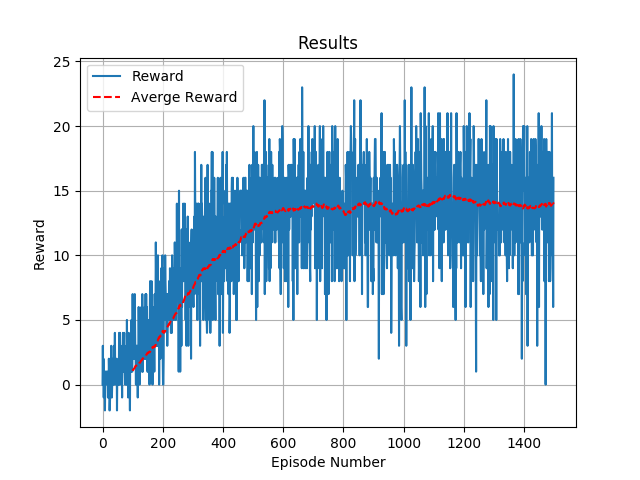
\includegraphics[width=0.8\linewidth]{./img/Results.png}
	\caption{Training results}
	\label{results}
\end{figure}



\section{Future Work}

\printbibliography
\end{document}
